\subsubsection{Mutation explorations in the network} \label{Sec:N_I:gene_sel}

Now most of the work done is exploratory, representing tools developed to understand how the mutations affect the network on RNAseq data. One result that I think is worth writing up is how important is the selection of genes. The story for this might be:
\begin{itemize}
    \item Starting point:
          \begin{itemize}
              \item The top 4000 genes with the highest median/std score were selected
              \item With this configuration there were small changes between communities after applying the modifiers
          \end{itemize}
    \item Representation of mutations in the selected genes see \ref*{fig:N_I:gene_sel}:
          \begin{itemize}
              \item How many of these genes are mutated? What is the distribution of the mutation count?
              \item How many of the genes mutated are not included in this selection
          \end{itemize}
    \item Problem:
          \begin{itemize}
              \item The selection of the genes prioritises the genes' variability but it mises on genes' magnitude and mutation frequency
              \item By prioritising variation over magnitude, we may miss genes that have a consistent high expression across multiple samples and are also mutated, e.g., FGFR3
          \end{itemize}
    \item Conclusion:
          \begin{itemize}
              \item We need to improve the way on how to select the genes: include both magnitude \& variance for gene expression and mutation count.
          \end{itemize}
\end{itemize}

I can think of two ways to improve the gene selection:
\begin{enumerate}
    \item Give PGCNA more genes and thus remove the variance bias.
          \begin{itemize}
              \item Pros: Quick, easy, no other biases introduced
              \item Cons: Messy, hard to analyse and to isolate the signal from the noise
          \end{itemize}
    \item Improve the selection mechanism:
          \begin{itemize}
              \item Pros: If done correctly it will represent a finding itself
              \item Cons: It will take longer, prone to introduce other biases (How do we prioritise magnitude vs variance vs mutation?)
          \end{itemize}
\end{enumerate}

On the discussion on how to prioritise magnitude vs variance vs mutations:
\begin{itemize}
    \item Ultimately the magnitude of TPM (gene expression) is the (proxy) method to determine the proteins which are the ones that dictate what's happening in the tissue.
    \item The variance is useful to identify the genes that vary, thus who may be very different between sample\_1 and sample\_2
    \item Mutation count is very important when the gene is consistently highly expressed (high magnitude) and for genes that vary. However, it has no significance when there is no expression of the gene mutated
\end{itemize}


Notes:
\begin{itemize}
    \item Score of variance – median/std
    \item Score for magnitude – percentile or the normalised value
    \item Score for mutations – normalised value
\end{itemize}


\paragraph{Checkpoint}
Based on the points from above, it feels that mutations have a lesser role than the magnitude and variance of a gene, that is because mutations are dependent for a gene to be expressed. Therefore, I will suggest the two sets of experiments:
\begin{todolist}
    \item Highest variance x highest magnitude
    \item Highest variance x highest magnitude x highest mutations
\end{todolist}


\paragraph{Draft Figures}

\begin{figure}
    \captionsetup[subfigure]{justification=Centering}
    \begin{subfigure}[t]{0.75\textwidth}
        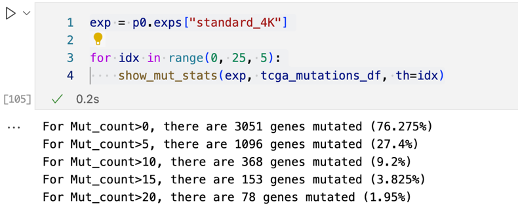
\includegraphics[width=\textwidth]{Sections/Network_I/Resources/Gene_selection/included_mut.png}
        \caption{Mutated genes in the selection}
    \end{subfigure}\hspace{\fill} % maximize horizontal separation

    \bigskip % more vertical separation
    \begin{subfigure}[t]{0.75\textwidth}
        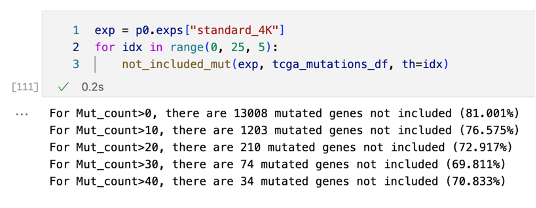
\includegraphics[width=\linewidth]{Sections/Network_I/Resources/Gene_selection/not_included_mut.png}
        \caption{Non-mutated genes in the selection}
    \end{subfigure}\hspace{\fill} % maximize horizontal separation

    \caption{Which of the genes are mutated and not in the selected genes}
    \label{fig:N_I:gene_sel}
\end{figure}
